\begin{figure*}
\centering
\subfloat[Group 1]{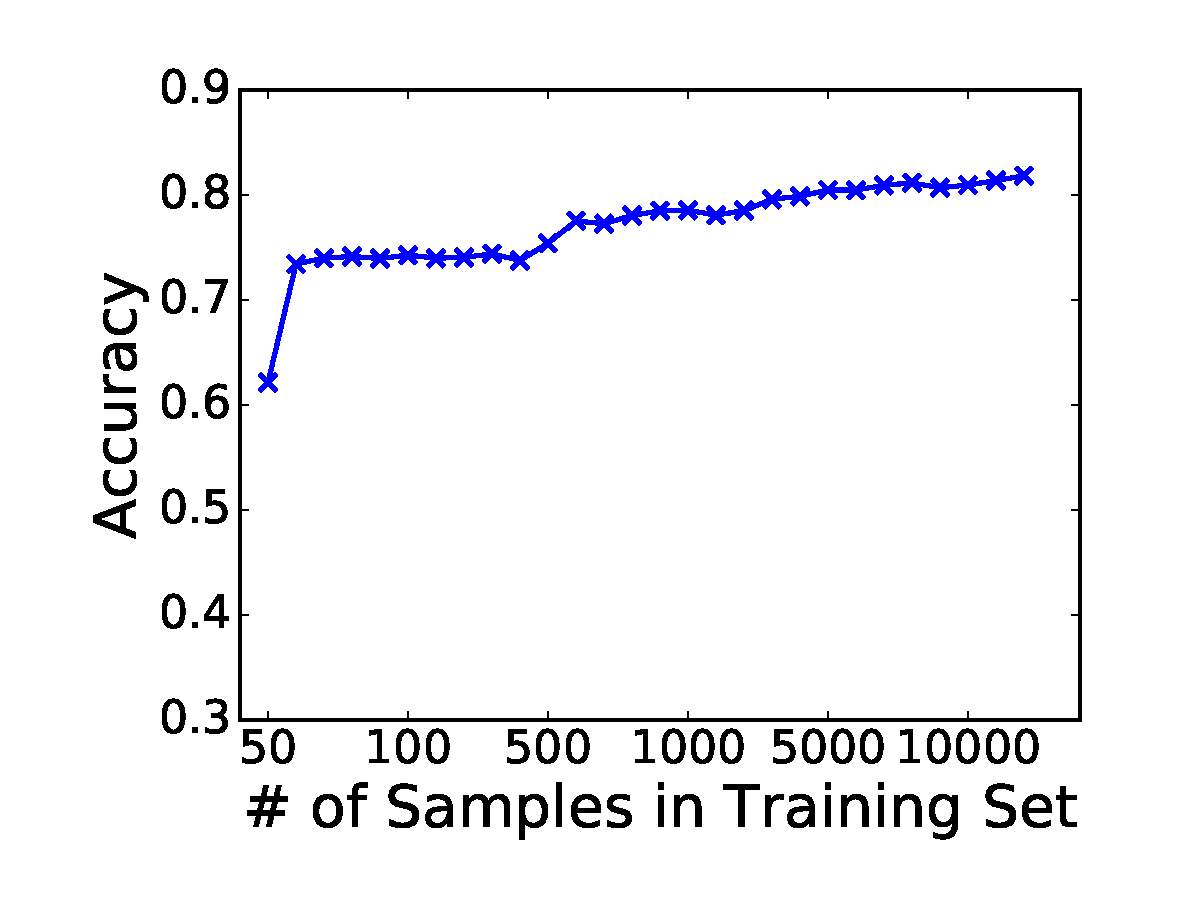
\includegraphics[width=0.16\linewidth]{figure/svm/0}\label{fig:moredata1}} 
\subfloat[Group 2]{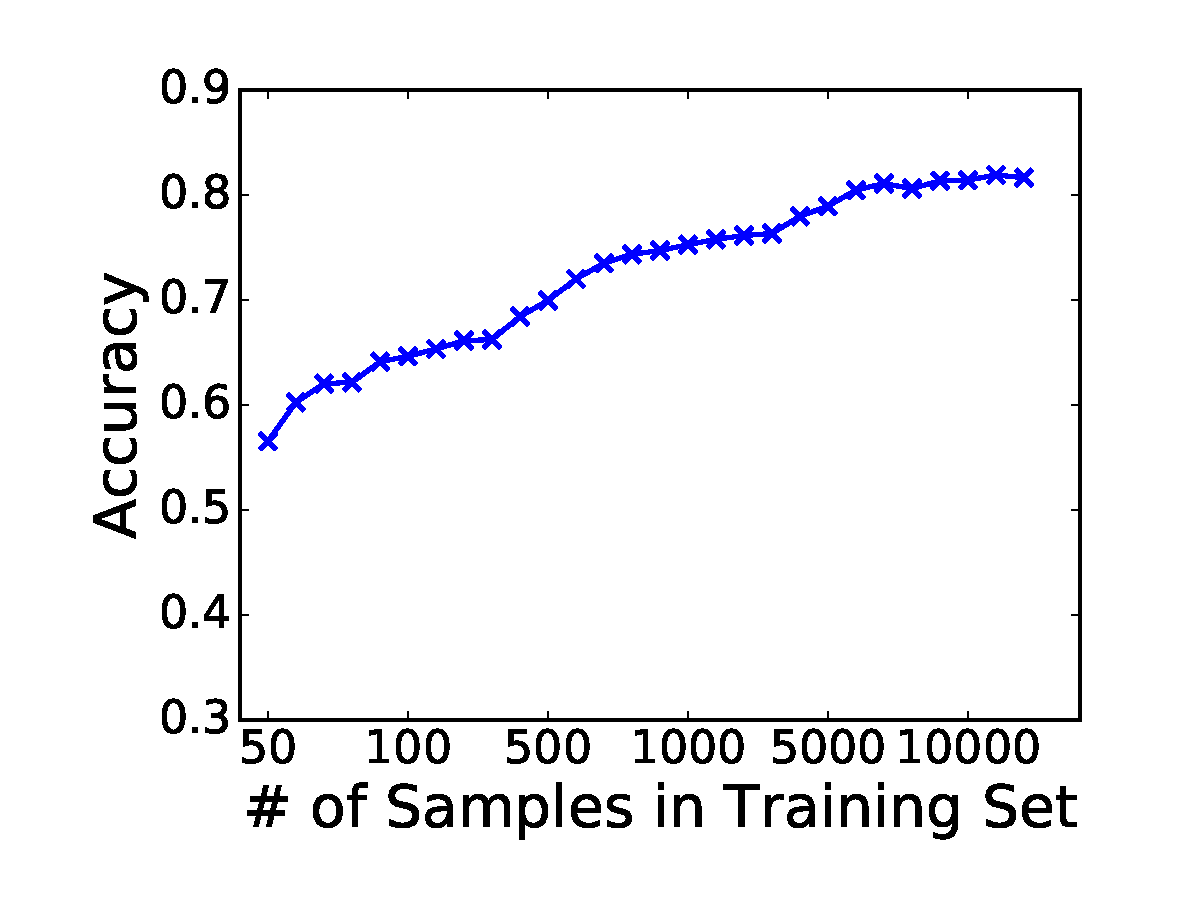
\includegraphics[width=0.16\linewidth]{figure/svm/1}\label{fig:moredata2}}
\subfloat[Group 3]{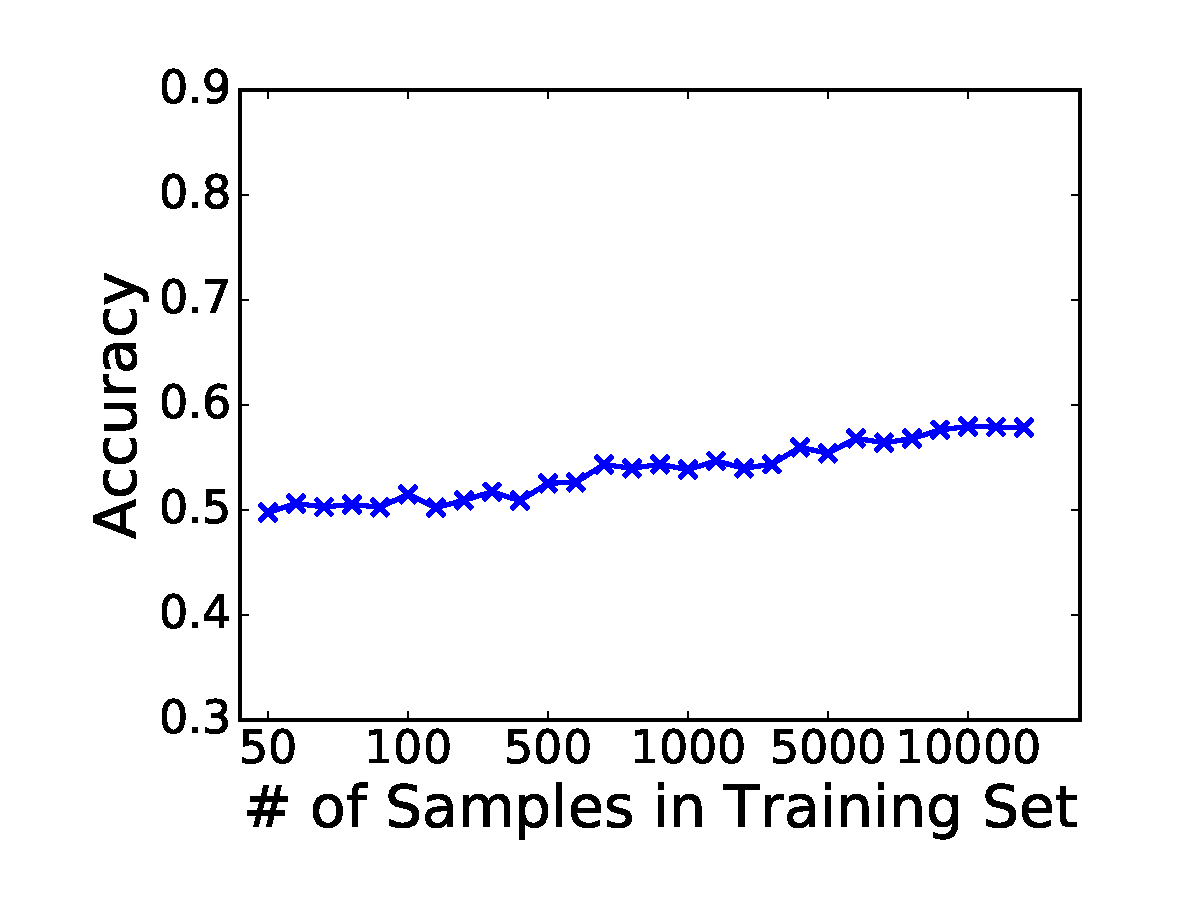
\includegraphics[width=0.16\linewidth]{figure/svm/2}\label{fig:moredata3}} 
\subfloat[Group 4]{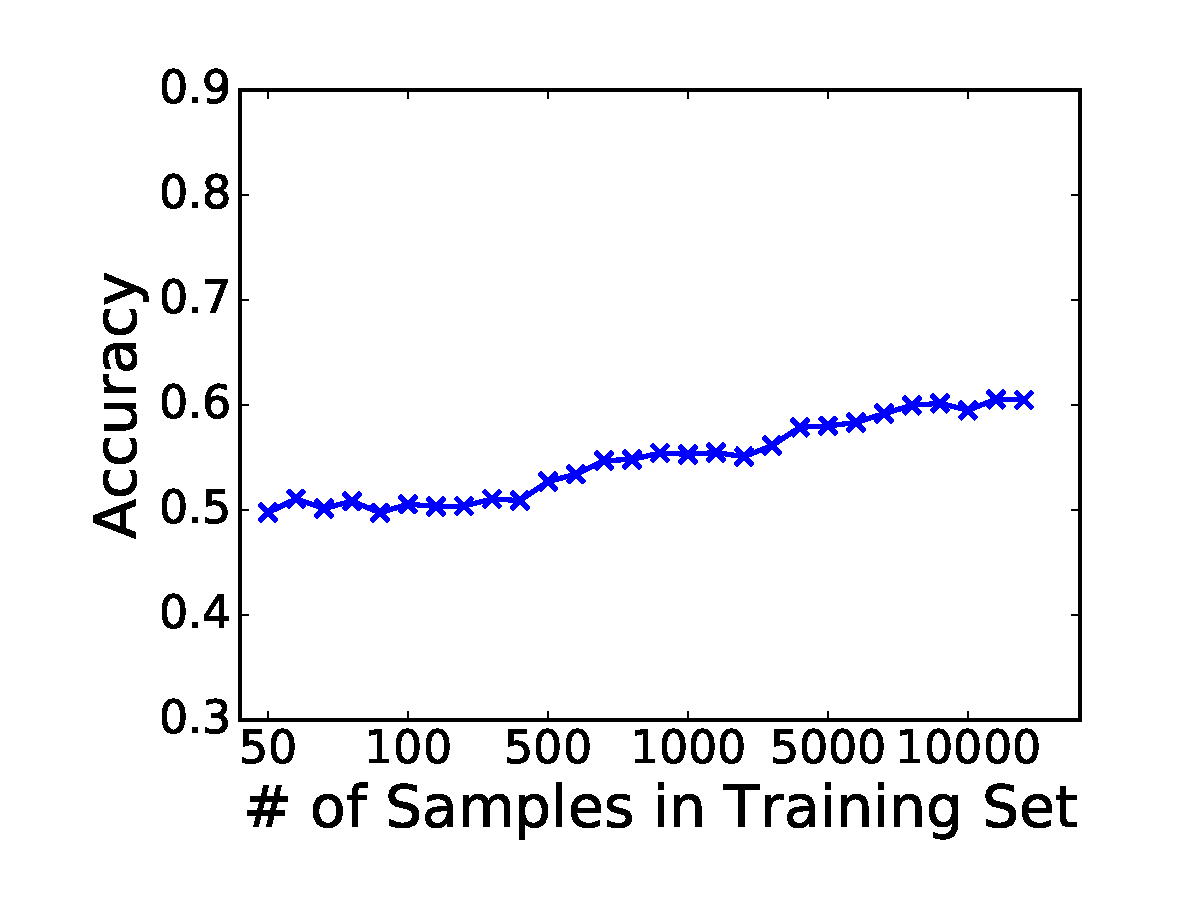
\includegraphics[width=0.16\linewidth]{figure/svm/3}\label{fig:moredata4}}
\subfloat[Group 5]{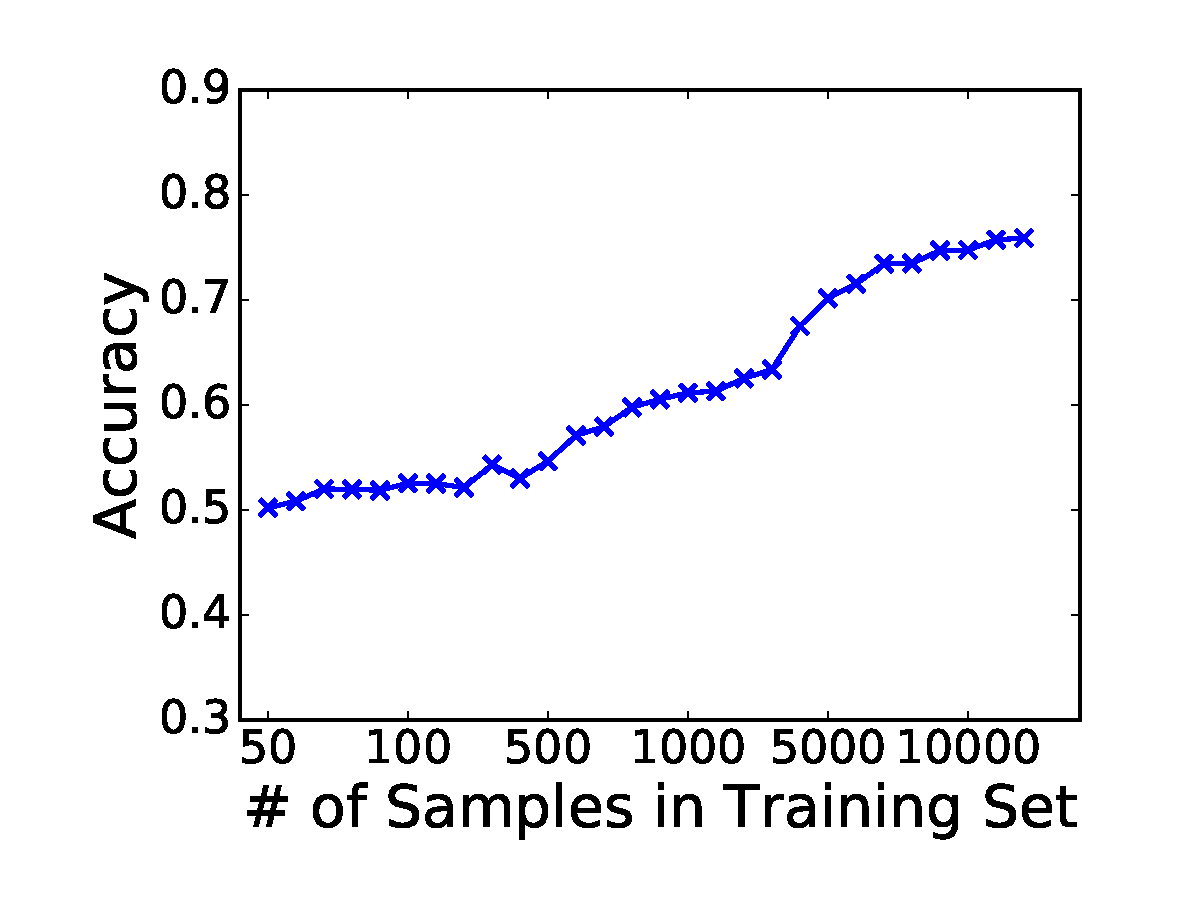
\includegraphics[width=0.16\linewidth]{figure/svm/4}\label{fig:moredata5}} \\ 

\subfloat[Group 6]{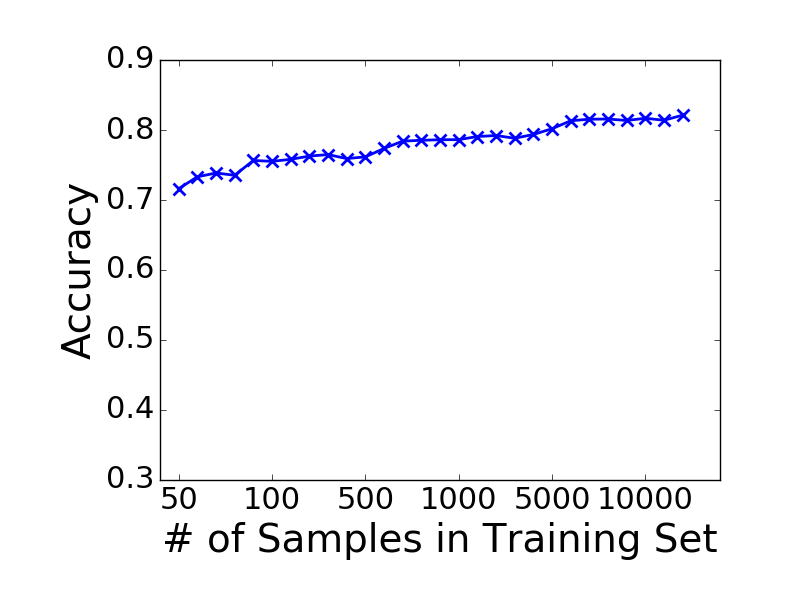
\includegraphics[width=0.16\linewidth]{figure/svm/5}\label{fig:moredata6}} 
\subfloat[Group 7]{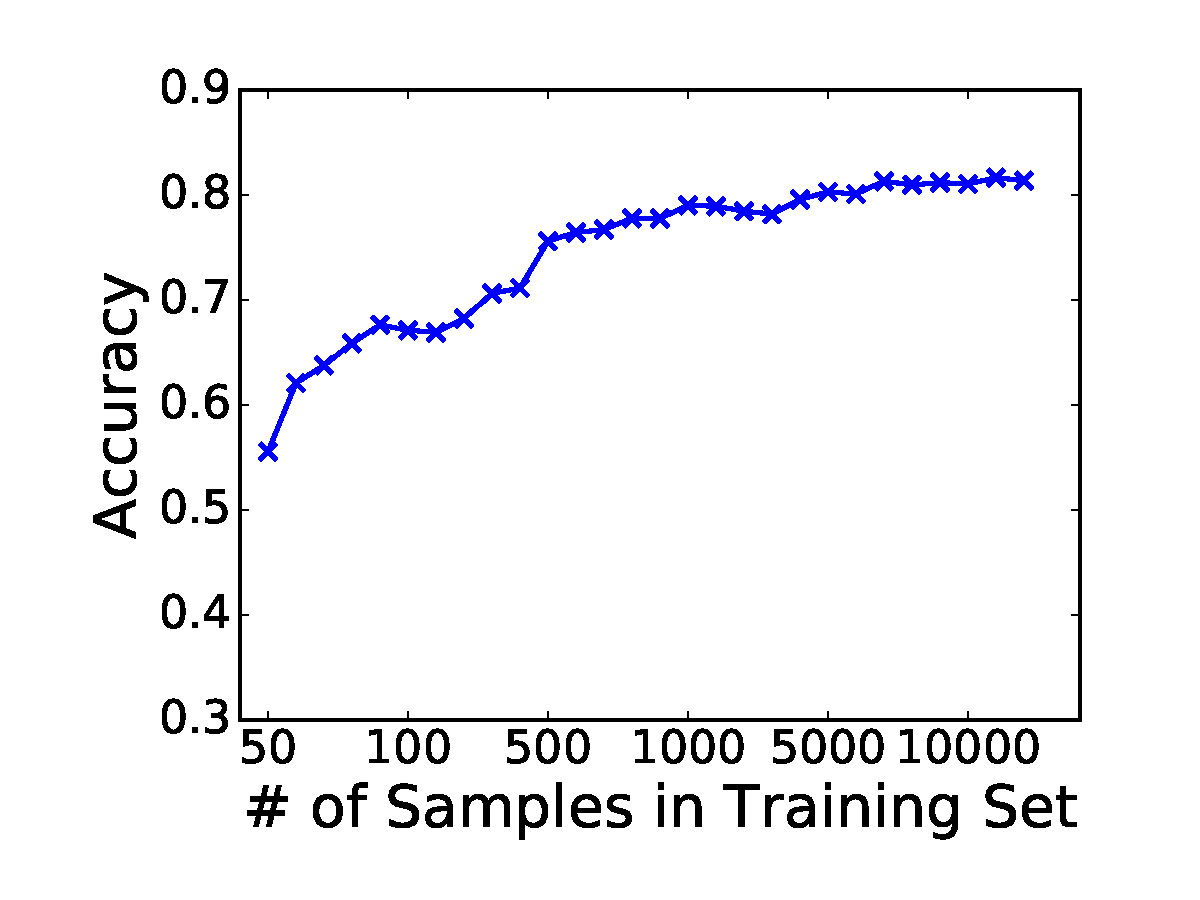
\includegraphics[width=0.16\linewidth]{figure/svm/6}\label{fig:moredata7}}
\subfloat[Group 8]{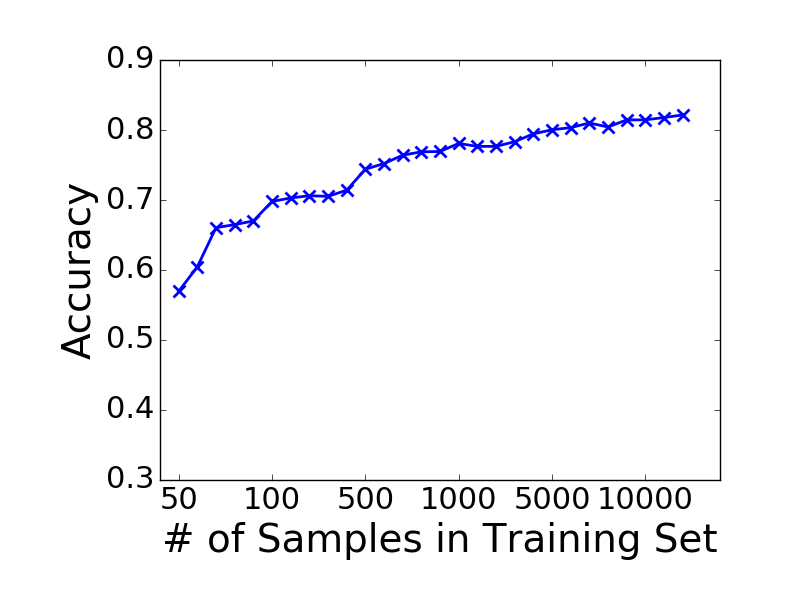
\includegraphics[width=0.16\linewidth]{figure/svm/7}\label{fig:moredata8}} 
\subfloat[Group 9]{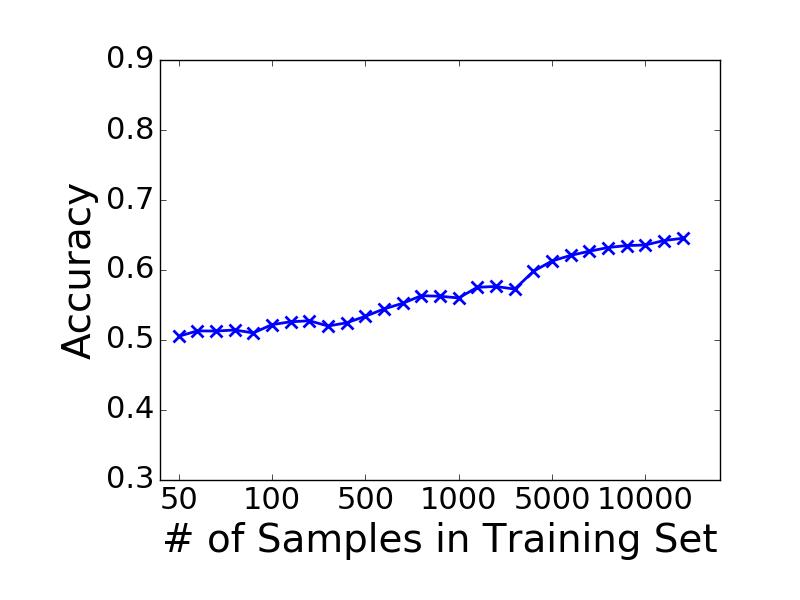
\includegraphics[width=0.16\linewidth]{figure/svm/8}\label{fig:moredata9}}
\subfloat[Group 10]{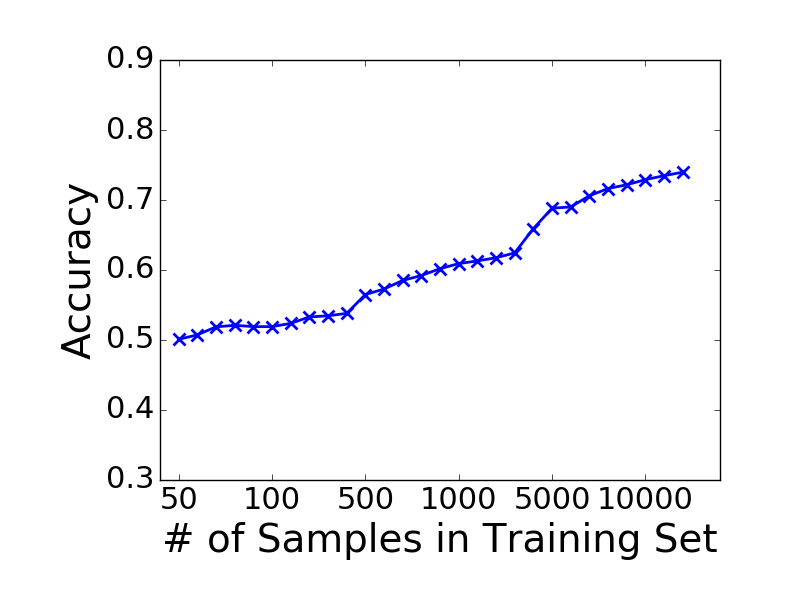
\includegraphics[width=0.16\linewidth]{figure/svm/9}\label{fig:moredata10}}
\subfloat[10-class]{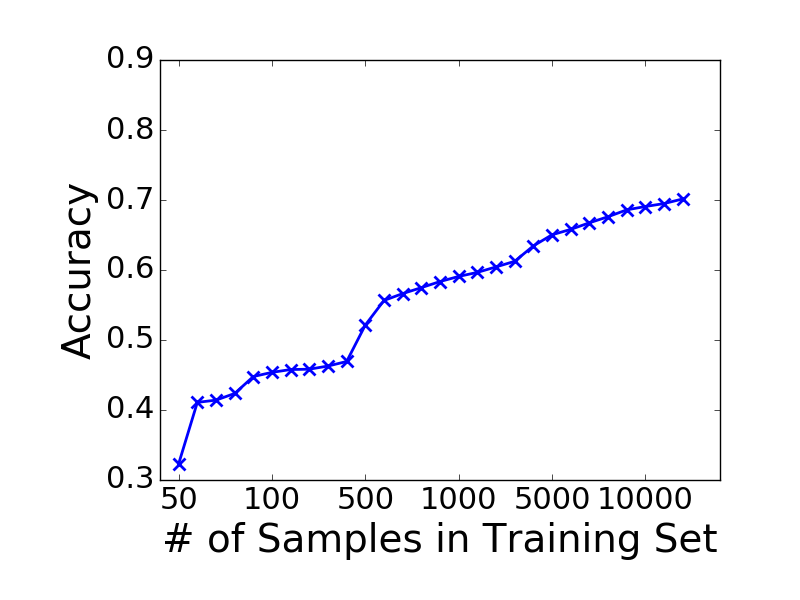
\includegraphics[width=0.16\linewidth]{figure/svm/10}\label{fig:moredata11}}
\caption{How accuracy changes with more data in traning set. 
{\footnotesize{(Figure~\ref{fig:moredata1} - Figure~\ref{fig:moredata10} show how accuracy of each two-class classifier changes 
with the size of training set changing from 50 to 10000. 
Figure~\ref{fig:moredata11} shows how accuracy of the ten-class classifier changes with the size of training set increaing from 50 to 10000. 
For all figures, the range of Y-axis is from 0.3 to 0.9.)}}} 
\label{fig:moredata} 
\end{figure*} 